\documentclass{beamer}
\usetheme{PaloAlto}
\usepackage{float}
\usecolortheme{whale}
\title[Simulating Valleytronics Logic at the Gate Level] % (optional, only for long titles)
{Simulating Valleytronics Logic at Gate Level}
\subtitle{A C++ Library and Example for Building Fully Electric Valleytronic Processors}
\author[] % (optional, for multiple authors)
{T. Jacovich\inst{1}}
\institute[Universities Here and There] % (optional)
{
 % \inst{1}%
  %Department of Electrical and Computer Engineering\\
  %The George Washington University
  %\and
  \inst{1}%
  Department of Physics\\
  The George Washington University
}
\date[AM2018] % (optional)
{ECE 6120: Advanced Microarchitecture Final Presentation}
\subject{Computer Science}
\begin{document}
\frame{\titlepage}
  \section[Introduction]{Introduction}
  \begin{frame}
    \frametitle{Valleytronics vs. CMOS}
    \small CMOS logic takes advantage of the Pauli Exclusion principle to create diodes and transistors. These allow easy voltage manipulation, but no additional constraints. Valleytronics offers a more precise view of the electron, in a manner similar to spintronics.  Valleytronics has the following unique attributes.

    \begin{itemize}
    \item[$\bullet$] Uses momentum states present in the metal (called valley states) to record additional information.
    
  \item[$\bullet$] Can be used in both classical and quantum processes depending on the implementation
  
  \item[$\bullet$] Incredibly new technology (Some of the required solid state metals were discovered in the last 5 years)
\end{itemize}
\vspace*{20pt}
 
\vspace*{20pt}
  \end{frame}
  
    \subsection[Warning: Quantum Physics]{QM}
    \begin{frame}
    \frametitle{The Physics Behind All electronic gates}

\begin{itemize}
  \item[$\bullet$]Most realizations involving valleytronics have involved ultra-cold states to generate the effects.
  
  \item[$\bullet$]They have also required lasers or intense magnetic fields to create and modify
  
  \item[$\bullet$]The presented gates are based off of Ang et al. (Phys Rev. B 96, 245410 2017)
  
 \item[$\bullet$ ]These gates take advantage of \textit{pseudospin-assisted valley-contrasted quantum-tunneling} (Yeah that is really what it is called.)  Referred to as 2MDS in the paper.
 
\end{itemize}

\end{frame}
  
   \begin{frame}
    \frametitle{The Physics Behind All-Electronic Gates}
   \framesubtitle{Schematics of the Gates}

  \begin{tabular}{cc}
  \begin{figure}
  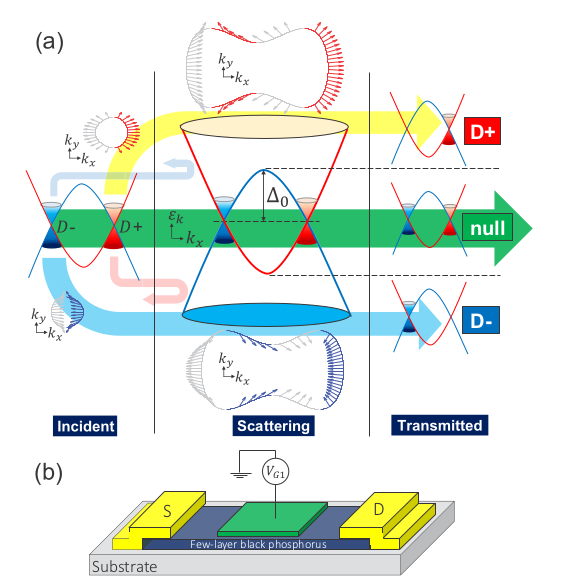
\includegraphics[scale=0.25]{gate_and_cones.png} 
  \end{figure}&   \begin{figure}
  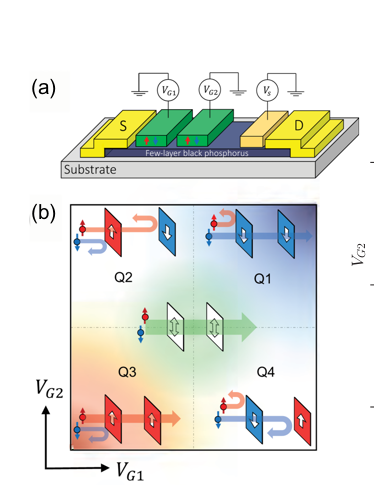
\includegraphics[scale=0.35]{gate1.png} 
  \end{figure} \
  \end{tabular}
\end{frame}
 
\section[Reversible Logic]{Reversible}
\begin{frame}
\frametitle{Reversible Logic}
\framesubtitle{The Landauer Limit and Beyond}
\begin{itemize}
\item[$\bullet$] One of the big advantages of this gate design is that it can be reversed with no additional logic.
\

\item[$\bullet$] This makes them interesting for quantum/classical hybrid machines and for reducing heat output because  of the Landauer Limit $\larrow k_{B}Tln\left[2\right]$ per lost bit.
\end{itemize}
\begin{figure}
  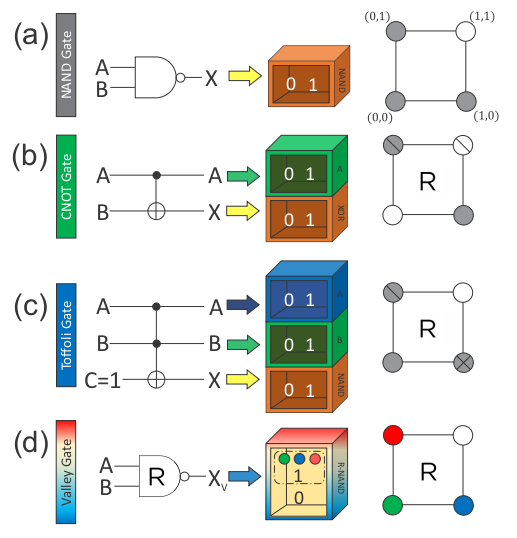
\includegraphics[scale=0.25]{full_gate.png} 
  \end{figure} \
\end{frame}

\section[The Plan]{The Plan}
\begin{frame}
\frametitle{The Plan}

\begin{itemize}
  \item[$\bullet$]The Original Plan was to take one of the readily available MIPS simulators and modify it to support valleytronic logic.
  \vspace*{10pt}
  \item[$\bullet$]The original plan was to implement the gates as close to physically accurate as possible.
  \vspace{10pt}
  \item[$\bullet$]Because the MIPS simulator already simulated a processor, it seemed straightforward to compare valleytronic and traditional boolean logic
 \vspace{10pt}
\item[$\bullet$] But did this actually come to pass? 
\end{itemize}

\end{frame}

\section[The Reality]{The Reality}
\begin{frame}
\frametitle{The Reality}

\begin{itemize}
  \item[$\bullet$]Trying to physically simulate the logic based on the Dirac Equation was Dumb (and slow, and ineffective).
  \vspace*{10pt}
  \item[$\bullet$]Only a few MIPS processor go down to individual gates and are available to be parsed at the level I needed, and they didn't like the 2 bits of information per single signal
  \vspace{10pt}
  \item[$\bullet$]VHDL based simulators let me define some of the gates, but the valleytronic were not easily passed about.
 \vspace{10pt}
\item[$\bullet$] So I ended up starting from scratch in C++
\end{itemize}

\end{frame}

\section[valleytronics\_logic]{valleytronics\_logic}
\begin{frame}
\frametitle{\texttt{valleytronics\_logic}}
\begin{itemize}
  \item[$\bullet$]A collection of libraries containing two classes \texttt{c\_valley} (logic gates)\texttt{ c\_vlogic}(more complex circuits)
  \vspace*{10pt}
  \item[$\bullet$]c\_valley contains most major logic gates to produces larger circuits as member objects.  The rest can be constructed from these gates.
  \vspace{10pt}
  \item[$\bullet$]c\_vlogic contains several pieces of logic that operate reversibly.
 \vspace{10pt}
\item[$\bullet$]Unfortunately there are no CPU simulations yet because flip-flops and latches that preserve the valley polarization are not trivial.
\end{itemize}

\end{frame}

\section[Results and Conclusions]{R and C}
\begin{frame}
\frametitle{Results and Conclusions}
\begin{itemize}
  \item[$\bullet$]All electric valleytronics could represent the next major logic technology
  \vspace*{10pt}
  \item[$\bullet$] As such, being able to readily simulate the logic is important for understanding where microarchitecure may be headed.
  \vspace{10pt}
  \item[$\bullet$]Although there are currently some major hurdles, \texttt{valleytronics\_logic} could conceivably serve as the basis for that next step. 
 \vspace{10pt}
\item[$\bullet$]The big thing would be cycle logic, and that is not too far away, just further away than this presentation deadline.
\end{itemize}

\end{frame}

\section[References]{References}
\begin{frame}
\frametitle{References}
\begin{itemize}
\item[1] Ang et al. Phys Rev B 96, 245410 (2017)

\vspace*{30pt}
\item[2]Isberg et al. Nature Materials 12 14/06/2013

\vspace*{100pt}
\end{itemize}


\end{frame}

\end{document}